\documentclass[fleqn, a4paper, 12pt, twoside]{article}
\usepackage{exsheets} %question and solution environments
\usepackage{amsmath, amssymb, amsthm} %standard AMS packages
\usepackage{esint} %integral signs
\usepackage{marginnote} %marginnotes
\usepackage{gensymb} %miscellaneous symbols
\usepackage{commath} %differential symbols
\usepackage{xcolor} %colours
\usepackage{cancel} %cancelling terms
\usepackage{siunitx} %formatting units
\usepackage{tikz, pgfplots} %diagrams
	\usetikzlibrary{calc, hobby, patterns, intersections, angles, quotes, spy}
\usepackage{graphicx} %inserting graphics
\usepackage{epstopdf} %converting and inserting eps graphics
\usepackage{hyperref} %hyperlinks
\usepackage{datetime} %date and time
\usepackage{ulem} %underline for \emph{}
\usepackage{xfrac, lmodern} %inline fractions
\usepackage{enumerate, enumitem} %numbered lists
\usepackage{float} %inserting floats
\usepackage[american voltages]{circuitikz} %circuit diagrams
\usepackage{pdflscape} %pages in landscape orientation
\usepackage{setspace} %double spacing
\usepackage{microtype} %micro-typography
\usepackage{listings} %formatting code
	\lstset{language=Matlab}
	\lstdefinestyle{standardMatlab}
	{
		belowcaptionskip=1\baselineskip,
		breaklines=true,
		frame=L,
		xleftmargin=\parindent,
		language=C,
		showstringspaces=false,
		basicstyle=\footnotesize\ttfamily,
		keywordstyle=\bfseries\color{green!40!black},
		commentstyle=\itshape\color{purple!40!black},
		identifierstyle=\color{blue},
		stringstyle=\color{orange},
	}
\usepackage{algpseudocode} %algorithms
\usepackage{algorithm} %algorithms

\renewcommand{\marginfont}{\scriptsize \color{red}}

\newcommand\numberthis{\addtocounter{equation}{1}\tag{\theequation}} %adds numbers to specific equations in non-numbered list of equations

\theoremstyle{definition}
\newtheorem{example}{Example}
\newtheorem{definition}{Definition}

\theoremstyle{theorem}
\newtheorem{theorem}{Theorem}
\newtheorem{law}{Law}

\newcommand{\curl}{\mathrm{curl\,}}

\newcommand{\divergence}{\mathrm{div\,}}

\makeatletter
\@addtoreset{section}{part} %resets section numbers in new part
\makeatother

\newcommand\blfootnote[1]{%
	\begingroup
	\renewcommand\thefootnote{}\footnote{#1}%
	\addtocounter{footnote}{-1}%
	\endgroup
}

\renewcommand{\tilde}{\widetilde}

\SetupExSheets{solution/print = true} %prints all solutions by default

%opening
\title{Harmonic Analysis}
\author{Aakash Jog}
\date{2015-16}

\begin{document}

\maketitle
%\setlength{\mathindent}{0pt}

\blfootnote
{	
	\begin{figure}[H]
		
\includegraphics[height = 12pt]{cc.eps}
		\includegraphics[height = 12pt]{by.eps}
		\includegraphics[height = 12pt]{nc.eps}
		\includegraphics[height = 12pt]{sa.eps}
	\end{figure}
	This work is licensed under the Creative Commons Attribution-NonCommercial-ShareAlike 4.0 International License. To view a copy of this license, visit \url{http://creativecommons.org/licenses/by-nc-sa/4.0/}.
} %CC-BY-NC-SA license

\tableofcontents

\newpage
\section{Lecturer Information}

\textbf{Barak Sober}\\
~\\
Office: Shenkar Physics 201\\
E-mail: \href{mailto:barakino@gmail.com}{barakino@gmail.com}\\
Telephone: \href{tel:+972 3-640-6024}{+972 3-640-6024}

\section{Required Reading}

\begin{enumerate}
	\item Folland, G.B.: Fourier Analysis and its applications, Wadsworth \& Brooks/Cole mathematics series, 1992
\end{enumerate}

\section{Additional Reading}

\begin{enumerate}
	\item Katznelson, Yitzhak. An introduction to Harmonic analysis. Cambridge University Press, 2004.
\end{enumerate}

\newpage
\part{Basic Definitions and Theorems}
\section{Sequences and Series}

\begin{definition}[Convergent series]
	The series $\sum\limits_{n = 0}^{\infty} a_n$ is said to converge if the sequence of partial sums $S_N = \sum\limits_{n = 0}^{N} a_n$ converges to a finite limit.
\end{definition}

\begin{definition}[Pointwise convergence of sequence of functions]
	Let $D \subseteq \mathbb{R}$, and $\{f_n(x) : D \to \mathbb{R}\}$ be a sequence of functions.
	$f_n(x)$ is said to converge pointwise, to a limit function $f(x)$ on $D$, if $\forall \varepsilon > 0$, $\forall x \in D$, $\exists N \in \mathbb{N}$, such that $\forall n > N$, $\left| f_n(x) - f(x) \right| < \varepsilon$.
\end{definition}

\begin{definition}[Uniform convergence of sequence of functions]
	Let $D \subseteq \mathbb{R}$, and $\{f_n(x) : D \to \mathbb{R}\}$ be a sequence of functions.
	$f_n(x)$ is said to converge uniformly to $f(x)$ on $D$< if $\forall \varepsilon > 0$, $\exists N \in \mathbb{N}$, such that, $\forall n > N$, $\forall x \in D$, $\left| f_n(x) - f(x) \right| < \varepsilon$.
\end{definition}

\begin{theorem}
	If $\left\{ f_n(x) \right\}_{n = 1}^{\infty}$ are continuous functions, and $f_n(x) \xrightarrow{U} f(x)$, then $f(x)$ is also continuous.
\end{theorem}

\begin{theorem}
	If a sequence of functions converges pointwise as well as uniformly, then the limit function must be the same.
\end{theorem}

\begin{theorem}[Weierstrass M-test]
	If $|u_k(x)| \le c_k$ on $D$ for $k \in \{ 1, 2, 3, \dots \}$ and the numerical series $\sum\limits_{k = 1}^{\infty} c_k$ converges, then the series of functions $\sum\limits_{k = 1}^{\infty} u_k(x)$ converges uniformly on $D$.
	\label{Weierstrass_M-test}
\end{theorem}

\section{Periodic Functions}

\begin{definition}[Periodic functions]
	A function $f : \mathbb{R} \to \mathbb{R}$ is said to be periodic if $\exists 0 < L \in \mathbb{R}$, such that $\forall x \in \mathbb{R}$,
	\begin{align*}
		f(x) & = f(x + L)
	\end{align*}
	If there exists a minimum $L$, it is called $L^*$, the fundamental period.
	\marginnote
	{
		For a function $f(x) = k$, as any positive number is a period, there is no minimum $L$.
		Hence, $\nexists L^*$.
	}
\end{definition}

\section{Odd and Even Functions}


\begin{definition}[Odd functions]
	A function is said to be odd if $f(-x) = -f(x)$.
	\marginnote
	{
		Odd functions are symmeteric about the origin.
	}
\end{definition}

\begin{definition}[Even functions]
	A function is said to be even if $f(-x) = f(x)$.
	\marginnote
	{
		Odd functions are symmeteric about the $y$-axis.
	}
\end{definition}

\begin{theorem}
	If $h(x)$ is odd,
	\begin{align*}
		\int\limits_{-L}^{L} h(x) \dif x & = 0
	\end{align*}
\end{theorem}

\newpage
\part{Introduction to Fourier Series}

\section{Real Fourier Series}

\begin{definition}
	Let $f : [-L,L] \to \mathbb{R}$, where $L > 0$.
	If $\forall x \in [-L,L]$, then
	\begin{align*}
		f(x) & = \frac{1}{2} a_0 + \sum\limits_{n = 1}^{\infty} \left( a_n \cos\left( \frac{n \pi}{L} x \right) + b_n \sin\left( \frac{n \pi}{L} x \right) \right)
	\end{align*}
\end{definition}

\begin{theorem}
	Let $L > 0$, $m \in \mathbb{W}$, $n \in \mathbb{W}$.\\
	Then
	\begin{align*}
		\int\limits_{-L}^{L} \cos\left( \frac{m \pi}{L} x \right) \cos\left( \frac{n \pi}{L} x \right) \dif x &=
			\begin{cases}
				0   & ;\quad m \neq n     \\
				L   & ;\quad m = n \neq 0 \\
				2 L & ;\quad m = n = 0    \\
			\end{cases}
	\end{align*}
\end{theorem}

\begin{proof}
	\begin{align*}
		E & = \int\limits_{-L}^{L} \cos\left( \frac{m \pi}{L} x \right) \cos\left( \frac{n \pi}{L} x \right) \dif x \\
                  & = \int\limits_{-L}^{L} \frac{1}{2} \left( \cos\left( (m + n) \frac{\pi}{L} x \right) + \cos\left( (m - n) \frac{\pi}{L} x \right) \right) \dif x
		\marginnote{$\because \left( \cos \alpha \cos \beta = \frac{1}{2} \left( \cos(\alpha + \beta) + \cos(\alpha - \beta) \right) \right)$}
	\end{align*}
	If $m \neq n$,
	\begin{align*}
		E & = \frac{1}{2} \left. \left( \frac{\sin\left( (m + n) \frac{\pi}{L} x \right)}{(m + n) \frac{\pi}{L}} + \frac{\sin\left( (m - n) \frac{\pi}{L} x \right)}{(m - n) \frac{\pi}{L}} \right) \right|_{-L}^{L} \\
                  & = 0
	\end{align*}
	~\\
	If $m = n \neq 0$,
	\begin{align*}
		E & = \int\limits_{-L}^{L} \frac{1}{2} \left( \cos\left( 2 m \frac{\pi}{L} x \right) + 1 \right) \dif x                      \\
                  & = \frac{1}{2} \int\limits_{-L}^{L} \cos\left( 2 m \frac{\pi}{L} x \right) \dif x + \left. \frac{1}{2} x \right|_{-L}^{L} \\
                  & = L
	\end{align*}
	~\\
	If $m = n = 0$,
	\begin{align*}
		E & = \int\limits_{-L}^{L} \cos(0) \cos(0) \dif x \\
                  & = \left. x \right|_{-L}^{L}                   \\
                  & = 2 L
	\end{align*}
\end{proof}

\begin{theorem}
	Let $L > 0$, $m \in \mathbb{N}$, $n \in \mathbb{N}$.\\
	Then
	\begin{align*}
		\int\limits_{-L}^{L} \sin\left( \frac{m \pi}{L} x \right) \sin\left( \frac{n \pi}{L} x \right) \dif x &=
			\begin{cases}
				0 & ;\quad m \neq n \\
				L & ;\quad m = n    \\
			\end{cases}
	\end{align*}
\end{theorem}

\begin{theorem}
	Let $L > 0$, $m \in \mathbb{W}$, $n \in \mathbb{W}$.\\
	Then
	\begin{align*}
		\int\limits_{-L}^{L} \sin\left( \frac{m \pi}{L} x \right) \cos\left( \frac{n \pi}{L} x \right) \dif x & = 0
	\end{align*}
\end{theorem}

Assuming $f(x)$ is known, and assuming that it can be integrated term by term,
\begin{align*}
	\int\limits_{-L}^{L} f(x) \dif x            & = \int\limits_{-L}^{L} \frac{1}{2} a_0 \dif x + \sum_{n = 1}^{\infty} a_n \int\limits_{-L}^{L} \cos\left( n \frac{\pi}{L} x \right) \dif x + b_n \int\limits_{-L}^{L} \sin\left( n \frac{\pi}{L} x \right) \dif x \\
	\therefore \int\limits_{-L}^{L} f(x) \dif x & = \frac{1}{2} \int\limits_{-L}^{L} a_0 \dif x                                                                                                                                                                     \\
                                                    & = \frac{1}{2} a_0 \cdot 2 L                                                                                                                                                                                       \\
	\therefore a_0                              & = \frac{1}{L} \int\limits_{-L}^{L} f(x) \dif x
\end{align*}
Similarly, multiplying the series with $\cos\left( m \frac{\pi}{L} x \right)$ for $m \neq 0$ and integrating,
\begin{align*}
	a_m & = \frac{1}{L} \int\limits_{-L}^{L} f(x) \cos\left( m \frac{\pi}{L} x \right) \dif x
\end{align*}
for $m \in \mathbb{N}$.\\
Similarly, for $m \in \mathbb{N} \setminus \{0\}$,
\begin{align*}
	b_m & = \frac{1}{L} \int\limits_{-L}^{L} f(x) \sin\left( m \frac{\pi}{L} x \right) \dif x
\end{align*}

\begin{definition}
	The expansion
	\begin{align*}
		f(x) & \approx \frac{1}{2} a_0 + \sum\limits_{i = 1}^{\infty} \left( a_n \cos\left( n \frac{\pi}{L} x \right) + b_n \sin\left( n \frac{\pi}{L} x \right) \right)
	\end{align*}
	where, for $m \in \mathbb{N}$,
	\begin{align*}
		a_m & = \frac{1}{L} \int\limits_{-L}^{L} f(x) \cos\left( m \frac{\pi}{L} x \right) \dif x
	\end{align*}
	and, for $m \in \mathbb{N} \setminus \{0\}$,
	\begin{align*}
		b_m & = \frac{1}{L} \int\limits_{-L}^{L} f(x) \sin\left( m \frac{\pi}{L} x \right) \dif x
	\end{align*}
	is called the Fourier Series of $f(x)$.
\end{definition}

\section{Complex Fourier Series}

By Euler's formula,
\begin{align*}
	\cos \theta &= \frac{1}{2} \left( e^{i \theta} + e^{-i \theta} \right)\\
	\sin \theta &= \frac{1}{2 i} \left( e^{i \theta} - e^{-i \theta} \right)
\end{align*}
Therefore,
\begin{align*}
	\frac{1}{2 i} &= -\frac{i}{2}
\end{align*}
Therefore, substituting in the Fourier series,
\begin{align*}
	f(x) &\approx \frac{1}{2} a_0 + \sum\limits_{n = 1}^{\infty} \left( a_n \frac{1}{2} \left( e^{\frac{i n \pi}{L} x} + e^{-\frac{i n \pi}{L} x} \right) - b_n \frac{i}{2} \left( e^{\frac{i n \pi}{L} x} - e^{-\frac{i n \pi}{L} x} \right) \right)\\
	&\approx \frac{1}{2} a_0 + \sum\limits_{n = 1}^{\infty} \left( e^{\frac{i n \pi}{L} x} \left( \frac{1}{2} a_n - \frac{i}{2} b_n \right) + e^{-\frac{i n \pi}{L} x} \left( \frac{1}{2} a_n + \frac{i}{2} b_n \right) \right)\\
	&\approx \frac{1}{2} a_0 + \sum\limits_{n = 1}^{\infty} \left( e^{\frac{i n \pi}{L} x} \left( \frac{1}{2} a_n - \frac{i}{2} b_n \right) \right) + \sum\limits_{n = -\infty}^{1} \left( e^{\frac{i n \pi}{L} x} \left( \frac{1}{2} a_n + \frac{i}{2} b_n \right) \right)\\
	&\approx \sum\limits_{n = -\infty}^{\infty} c_n e^{\frac{i n \pi}{L} x}
\end{align*}

\subsection{Bessel's Inequality}

\begin{definition}[Piecewise continuous functions]
	$f : \mathbb{R} \to \mathbb{R}$ is said to be piecewise continuous if, for every finite interval $[a,b]$ there is a finite number of discontinuity points, and the one-sided limits at each of these points are also finite.
\end{definition}

\begin{definition}[Piecewise continuously differentiable functions]
	$f : \mathbb{R} \to \mathbb{R}$ is said to be piecewise continuously differentiable if it is piecewise continuous, and
	\begin{align*}
		\lim\limits_{h \to 0^+} \frac{f(x + h) - f(x^+)}{h} &< \infty
	\end{align*}
	and
	\begin{align*}
		\lim\limits_{h \to 0^-} \frac{f(x + h) - f(x^-)}{h} &< \infty
	\end{align*}
\end{definition}

\begin{theorem}[Bessel's Inequality]
	Let $f(x)$ be a piecewise continuous function defined on $[-L,L]$.
	Then
	\begin{align*}
		\frac{1}{2} {a_0}^2 + \sum\limits_{n = 1}^{\infty} {a_n}^2 + {b_n}^2 &\le \frac{1}{L} \int\limits_{-L}^{L} {f(x)}^2 \dif x
	\end{align*}
	\label{Bessel's_Inequality}
\end{theorem}

\end{document}
